\chapter{Background and Introduction}
\label{chEx}
\section{Examples}
Here are some references! \cite{Demlow2014, Grotjohn2014}
This is how you reference \Cref{ch1}.

Note: you have to run the following Typeset commands in this order to get the labels and references all correct: 
\\ pdfLaTex
\\ BibTex
\\ pdfLaTex
\\ pdfLaTex
\\ you can run them in other orders, but you need BibTex to be run after pdfLaTex has been run once, and you need to run pdfLaTex twice more after to update the TOC, etc
\section{This is a section}
\label{a section}
This is how you reference anything really \Cref{a section}

\begin{table} [ht]
	\centering
\begin{tabular}{*{2}{c}}
\textbf{Property} & \textbf{Approximate Value (at 300K)} \\ \hline \hline \\
Thermal conductivity & \SI{21.9}{\watt\per\centi\meter\per\kelvin} \\
Band gap & 5.47 eV \\
Carrier mobility (electron, Hall effect) & \SI{660}{\centi\meter\square\per\volt\per\second}\\
Carrier mobility (hole, Hall effect) & \SI{1650}{\centi\meter\square\per\volt\per\second}\\
Dielectric constant & 5.7 \\
Breakdown electric field strength & 10-\SI{20}{\mega\volt\per\centi\meter} \\
Intrinsic resistivity & \SI{1e13}{\ohm\centi\meter} \\
Mechanical hardness & \SI{90}{\giga\pascal}\\
Sound propagation velocity & \SI{17.5}{\kilo\meter\per\second}
\end{tabular}
	\caption{Some Properties of Single Crystal Diamond \cite{May2000,Teraji2006}, in a table that has numbers with units using the SI package}
\label{tbl:Properties} %This is how you label a table to reference it
\end{table}

Here, I reference \Cref{tbl:Properties} and here's an example about equations and variables:
Johnson \cite{Johnson1965} has shown that the product of the breakdown electric field, $E_B$, and the maximum carrier drift velocity, $v_s$, sets the limit of various transistor parameters for devices made of a specified material. The result is the Johnson figure of merit ($JFOM$), given in \Cref{eq:JFOM}.

\begin{equation}
	JFOM = \frac{E_B\,v_s}{2\pi}
	\label{eq:JFOM}
\end{equation}

The charge carrier transit time cut-off frequency in a transistor is defined by $f_{\text{transit}} = 1/(2\pi \tau_{\text{avg}})$, where $\tau_{\text{avg}}$ is the average time it takes a charge carrier moving at an average velocity $v_{\text{avg}}$ to travel the emitter-to-collector distance 

\subsection{a subsection}
\begin{figure}[ht]
	\centering
	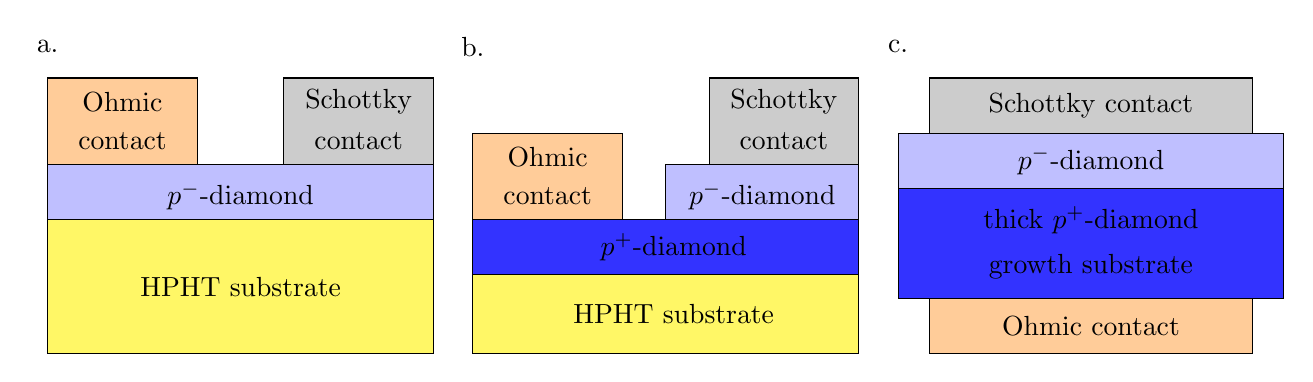
\begin{tikzpicture}

			\draw(-7.9,1.8) node{a.};
			\filldraw[fill=orange!40!white, draw=black] (-7.9,1.4) rectangle(-6,0.3); 
			\draw (-6.95,1.1) node{Ohmic}; 
			\draw (-6.95, 0.6) node{contact};
			\filldraw[fill=black!20!white, draw=black](-4.9,1.4) rectangle(-3,0.3); 
			\draw (-3.95,1.1) node{Schottky}; 
			\draw (-3.95,0.6) node{contact};
			\filldraw[fill=blue!25!white, draw=black] (-7.9,0.3) rectangle(-3,-0.4); 
			\draw (-5.45,-0.1) node{$p^{-}$-diamond};
\filldraw[fill=yellow!60!white, draw=black] (-7.9,-0.4) rectangle(-3,-2.1); 
			\draw (-5.45,-1.25) node{HPHT substrate};

			\draw(-2.5,1.8) node{b.};
			\filldraw[fill=orange!40!white, draw=black] (-2.5,0.7) rectangle(-0.6,-0.4); 
			\draw (-1.55,0.4) node{Ohmic}; 
			\draw (-1.55, -0.1) node{contact};
			\filldraw[fill=black!20!white, draw=black](0.5,1.4) rectangle(2.4,0.3); 
			\draw (1.45,1.1) node{Schottky}; 
			\draw (1.45,0.6) node{contact};
			\filldraw[fill=blue!25!white, draw=black] (-0.05,0.3) rectangle(2.4,-0.4); 
			\draw (1.175,-0.1) node{$p^{-}$-diamond};
			\filldraw[fill=blue!80!white, draw=black] (-2.5,-0.4) rectangle(2.4,-1.1); 
			\draw (0.05,-0.75) node{$p^{+}$-diamond};
\filldraw[fill=yellow!60!white, draw=black] (-2.5,-1.1) rectangle(2.4,-2.1); 
			\draw (0.05,-1.6) node{HPHT substrate};			

			\draw(2.9,1.8) node{c.};
			\filldraw[fill=black!20!white, draw=black](3.3,1.4) rectangle(7.4,0.7); 
			\draw (5.35,1.05) node{Schottky contact}; 
			\filldraw[fill=blue!25!white, draw=black] (2.9,0.7) rectangle(7.8,0.0); 
			\draw (5.35,0.35) node{$p^{-}$-diamond};
			\filldraw[fill=blue!80!white, draw=black] (2.9,0.0) rectangle(7.8,-1.4); 
			\draw (5.35,-0.4) node{thick $p^{+}$-diamond};
			\draw (5.35,-1) node{growth substrate};
\filldraw[fill=orange!40!white, draw=black] (3.3,-1.4) rectangle(7.4,-2.1); 
			\draw (5.35,-1.75) node{Ohmic contact};	

	\end{tikzpicture}
	\caption{You can draw figures with tikz For interpretation of the references to color in this and all other figures, the reader is referred to the electronic version of this thesis.}
	\label{fig:diodeArchitectures}
\end{figure}


\begin{figure}[ht]
	\centering
	\begin{tikzpicture}
\node(0,0)
 {\includegraphics[width=0.9\textwidth]{figures/ebandALL3.png}};

			\draw(-7.9,1.5) node{a.};
			\draw(-7.9,-.4) node{$E_{Fm}$};
			\draw (-3.45,0.7) node{$E_C$};
			\draw (-3.45,-0.37) node{$E_F$};
			\draw (-3.45,-0.8) node{$E_V$};
			\draw(-7.12,0.08) node{$q\phi_{Bp}$};
			\draw(-5.2,-1) node{$q\psi_{bi}$};
			\draw(-4,0.1) node{$q\phi_{p}$};

			\draw(-2.5,1.5) node{b.};
			\draw(-2.5,-.4) node{$E_{Fm}$};
			\draw (1.8,0.1) node{$E_C$};
			\draw (1.8,-0.78) node{$E_F$};
			\draw (1.8,-1.18) node{$E_V$};
			\draw(-1.8,0.02) node{$q\phi_{Bp}$};
			\draw(1,-1.8) node{$q(\psi_{bi}-V_F)$};
			\draw(0.4,-0.6) node{$qV_F$};

			\draw(2.75,1.5) node{c.};
			\draw(2.75,-.4) node{$E_{Fm}$};
			\draw (7.7,1.5) node{$E_C$};
			\draw (7.7,0.3) node{$E_F$};
			\draw (7.7,-0.15) node{$E_V$};
			\draw(3.52,0.02) node{$q\phi_{Bp}$};
			\draw(5.6,-0.9) node{$q(\psi_{bi} + V_R)$};
			\draw(7.15,-0.7) node{$qV_R$};
	\end{tikzpicture}
\caption{You can also draw over figures with tikz  \emph{Adapted from }\cite{Sze2006} }
\label{fig:bandbending}
\end{figure}

\begin{figure}[ht]
	\centering
	\includegraphics[width=0.4\textwidth]{figures/PH.jpg}
	\caption{Figures can be just pictures though}
	\label{fig:PH}
\end{figure}

\begin{figure}[h]
    \begin{center}
        \input{figures/ExampleConfocalScan.pgf}
    \end{center}
    \caption{A PGF confocal scan from \texttt{matplotlib}.}
\end{figure}